% Options for packages loaded elsewhere
\PassOptionsToPackage{unicode}{hyperref}
\PassOptionsToPackage{hyphens}{url}
\PassOptionsToPackage{dvipsnames,svgnames,x11names}{xcolor}
%
\documentclass[
  letterpaper,
  DIV=11,
  numbers=noendperiod,
  oneside]{scrartcl}

\usepackage{amsmath,amssymb}
\usepackage{iftex}
\ifPDFTeX
  \usepackage[T1]{fontenc}
  \usepackage[utf8]{inputenc}
  \usepackage{textcomp} % provide euro and other symbols
\else % if luatex or xetex
  \usepackage{unicode-math}
  \defaultfontfeatures{Scale=MatchLowercase}
  \defaultfontfeatures[\rmfamily]{Ligatures=TeX,Scale=1}
\fi
\usepackage{lmodern}
\ifPDFTeX\else  
    % xetex/luatex font selection
\fi
% Use upquote if available, for straight quotes in verbatim environments
\IfFileExists{upquote.sty}{\usepackage{upquote}}{}
\IfFileExists{microtype.sty}{% use microtype if available
  \usepackage[]{microtype}
  \UseMicrotypeSet[protrusion]{basicmath} % disable protrusion for tt fonts
}{}
\makeatletter
\@ifundefined{KOMAClassName}{% if non-KOMA class
  \IfFileExists{parskip.sty}{%
    \usepackage{parskip}
  }{% else
    \setlength{\parindent}{0pt}
    \setlength{\parskip}{6pt plus 2pt minus 1pt}}
}{% if KOMA class
  \KOMAoptions{parskip=half}}
\makeatother
\usepackage{xcolor}
\usepackage[left=1in,marginparwidth=2.0666666666667in,textwidth=4.1333333333333in,marginparsep=0.3in]{geometry}
\setlength{\emergencystretch}{3em} % prevent overfull lines
\setcounter{secnumdepth}{-\maxdimen} % remove section numbering
% Make \paragraph and \subparagraph free-standing
\makeatletter
\ifx\paragraph\undefined\else
  \let\oldparagraph\paragraph
  \renewcommand{\paragraph}{
    \@ifstar
      \xxxParagraphStar
      \xxxParagraphNoStar
  }
  \newcommand{\xxxParagraphStar}[1]{\oldparagraph*{#1}\mbox{}}
  \newcommand{\xxxParagraphNoStar}[1]{\oldparagraph{#1}\mbox{}}
\fi
\ifx\subparagraph\undefined\else
  \let\oldsubparagraph\subparagraph
  \renewcommand{\subparagraph}{
    \@ifstar
      \xxxSubParagraphStar
      \xxxSubParagraphNoStar
  }
  \newcommand{\xxxSubParagraphStar}[1]{\oldsubparagraph*{#1}\mbox{}}
  \newcommand{\xxxSubParagraphNoStar}[1]{\oldsubparagraph{#1}\mbox{}}
\fi
\makeatother


\providecommand{\tightlist}{%
  \setlength{\itemsep}{0pt}\setlength{\parskip}{0pt}}\usepackage{longtable,booktabs,array}
\usepackage{calc} % for calculating minipage widths
% Correct order of tables after \paragraph or \subparagraph
\usepackage{etoolbox}
\makeatletter
\patchcmd\longtable{\par}{\if@noskipsec\mbox{}\fi\par}{}{}
\makeatother
% Allow footnotes in longtable head/foot
\IfFileExists{footnotehyper.sty}{\usepackage{footnotehyper}}{\usepackage{footnote}}
\makesavenoteenv{longtable}
\usepackage{graphicx}
\makeatletter
\def\maxwidth{\ifdim\Gin@nat@width>\linewidth\linewidth\else\Gin@nat@width\fi}
\def\maxheight{\ifdim\Gin@nat@height>\textheight\textheight\else\Gin@nat@height\fi}
\makeatother
% Scale images if necessary, so that they will not overflow the page
% margins by default, and it is still possible to overwrite the defaults
% using explicit options in \includegraphics[width, height, ...]{}
\setkeys{Gin}{width=\maxwidth,height=\maxheight,keepaspectratio}
% Set default figure placement to htbp
\makeatletter
\def\fps@figure{htbp}
\makeatother

\KOMAoption{captions}{tableheading}
\makeatletter
\@ifpackageloaded{caption}{}{\usepackage{caption}}
\AtBeginDocument{%
\ifdefined\contentsname
  \renewcommand*\contentsname{Table of contents}
\else
  \newcommand\contentsname{Table of contents}
\fi
\ifdefined\listfigurename
  \renewcommand*\listfigurename{List of Figures}
\else
  \newcommand\listfigurename{List of Figures}
\fi
\ifdefined\listtablename
  \renewcommand*\listtablename{List of Tables}
\else
  \newcommand\listtablename{List of Tables}
\fi
\ifdefined\figurename
  \renewcommand*\figurename{Figure}
\else
  \newcommand\figurename{Figure}
\fi
\ifdefined\tablename
  \renewcommand*\tablename{Table}
\else
  \newcommand\tablename{Table}
\fi
}
\@ifpackageloaded{float}{}{\usepackage{float}}
\floatstyle{ruled}
\@ifundefined{c@chapter}{\newfloat{codelisting}{h}{lop}}{\newfloat{codelisting}{h}{lop}[chapter]}
\floatname{codelisting}{Listing}
\newcommand*\listoflistings{\listof{codelisting}{List of Listings}}
\makeatother
\makeatletter
\makeatother
\makeatletter
\@ifpackageloaded{caption}{}{\usepackage{caption}}
\@ifpackageloaded{subcaption}{}{\usepackage{subcaption}}
\makeatother
\makeatletter
\@ifpackageloaded{sidenotes}{}{\usepackage{sidenotes}}
\@ifpackageloaded{marginnote}{}{\usepackage{marginnote}}
\makeatother
\ifLuaTeX
  \usepackage{selnolig}  % disable illegal ligatures
\fi
\usepackage{bookmark}

\IfFileExists{xurl.sty}{\usepackage{xurl}}{} % add URL line breaks if available
\urlstyle{same} % disable monospaced font for URLs
\hypersetup{
  colorlinks=true,
  linkcolor={blue},
  filecolor={Maroon},
  citecolor={Blue},
  urlcolor={Blue},
  pdfcreator={LaTeX via pandoc}}

\author{}
\date{}

\begin{document}

\subsection{COMM 7018: Social Media
Theory}\label{comm-7018-social-media-theory}

\begin{figure}

\begin{minipage}{0.49\linewidth}
\href{http://polyducks.co.uk/}{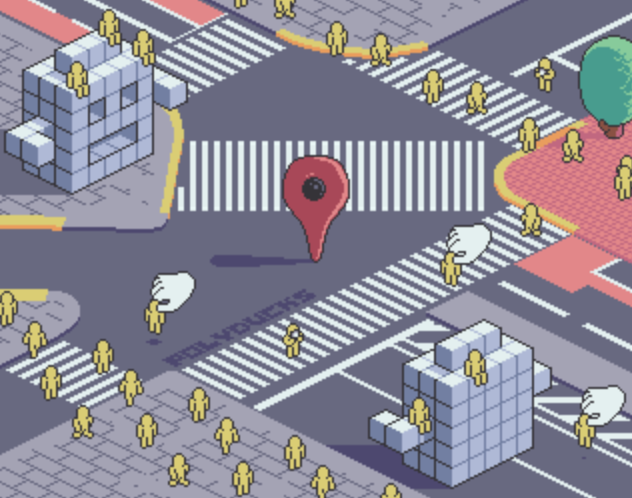
\includegraphics{img/polyducks.gif}}\end{minipage}%
%
\begin{minipage}{0.02\linewidth}
~\end{minipage}%
%
\begin{minipage}{0.49\linewidth}
\href{https://fitchburgstate.edu}{Fitchburg State University}\\
\href{https://www.fitchburgstate.edu/academics/academic-schools/school-arts-and-sciences/communications-media-department}{Communications
Media Department}\\
\href{https://www.fitchburgstate.edu/academics/programs/social-media-concentration-applied-communication-ms-online}{MS
in Applied Communication: Social Media Concentration}\\
GCE Online-Accelerated\\
7 weeks, Monday 22 May -- Sunday 9 July 2023\\
Instructor: Dr.~Martin Roberts\\
\href{https://mroberts1.github.io/social-media-theory-summer-2023}{Syllabus}\\
\href{https://github.com/mroberts1/social-media-theory-summer-2023}{GitHub
repository}\end{minipage}%

\end{figure}%

\begin{center}\rule{0.5\linewidth}{0.5pt}\end{center}

\paragraph{Overview}\label{overview}

The term \textbf{social media} is popularly understood as referring to
corporate-owned, advertising-funded communication \textbf{platforms}
based on \textbf{user-generated content}: YouTube, Instagram, Facebook,
Twitter, Twitch, Discord, TikTok. It can also be defined more broadly,
however, as a set of networked, technologically-mediated
\textbf{practices} of communication, structured by economic and
political forces that both inflect and are inflected by social and
cultural identities. These platforms, the social practices that they
enable, and the relationship between the two are the objects of
\textbf{social media theory}. But what does it mean to \textbf{theorize}
social media? Why do we need social media theory at all?

To theorize something involves a number of processes:

\begin{itemize}
\tightlist
\item
  first, how do we define the phenomenon or object of study itself? How
  does it differ from previous or other related phenomena?
\item
  how are we to account for it? Why did it happen/is it happening now
  rather than at some other time? What are its conditions of
  possibility?
\item
  what is its relation to larger areas of society? What are its
  implications for those areas?
\item
  how are we to evaluate it, in terms of its implications (political,
  economic, social, ethical, legal, environmental, aesthetic)? What are
  its possibilities and limits, its progressive and oppressive aspects?
  How can we change it for the better?
\end{itemize}

These processes involve developing analytical frameworks or models
comprising concepts that are useful for identifying and analyzing key
aspects of and issues raised by the phenomenon/object in question. These
frameworks and concepts typically draw from existing ones in different
fields of study, but often involve the proposal of new frameworks and
concepts specific to the field in question.

\begin{center}\rule{0.5\linewidth}{0.5pt}\end{center}

\paragraph{Objectives}\label{objectives}

By the end of the course, students will be able to:

\begin{itemize}
\tightlist
\item
  analyze technologies past, present, and imagined
\item
  describe the ways in which technologies shape our world the ways in
  which we shape those technologies
\item
  explain how social media is a result of the intersection between
  technologies and existing human communication dynamics
\item
  discuss how theory of technology and social media can improve the
  vocational outlook of a student
\item
  play a productive role in and facilitate conversations that tease out
  the relationships between values and technology.\\
\item
  through the skills you will refine in writing your research papers,
  clearly explain how a specific technology shapes the social world that
  we live in.
\end{itemize}

\begin{center}\rule{0.5\linewidth}{0.5pt}\end{center}

\paragraph{Course Texts}\label{course-texts}

These sources are either available online or excerpts will be posted on
Blackboard.

\begin{itemize}
\item
  \href{https://en.wikipedia.org/wiki/Amy_S._Bruckman}{Amy Bruckman},
  \emph{Should You Believe Wikipedia? Online Communities and the
  Construction of Knowledge}. Cambridge: Cambridge University Press,
  2022. \href{bruckman-refs.html}{References page}
\item
  Claire Dederer, \emph{Monsters: A Fan's Dilemma}. New York: Alfred A.
  Knopf, 2023.
\item
  \href{https://mssv.net/}{Adrian Hon}, \emph{You've Been Played: How
  Corporations, Governments, and Schools Use Games to Control Us All}.
  New York: Basic Books, 2022.
\item
  Cathy O'Neil, with Stephen Baker, \emph{The Shame Machine: Who Profits
  in the New Age of Humiliation}. New York: Crown/Random House, 2022.
\item
  \href{https://allissavrichardson.com}{Allissa V. Richardson},
  \emph{Bearing Witness While Black: African Americans, Smartphones, and
  the New Protest \#Journalism} (Oxford: Oxford University Press, 2020).
\item
\item
  Maggie Appleton, ``\href{https://maggieappleton.com/cozy-web}{The Dark
  Forest \& The Cozy Web}''
\item
\item
  Yancey Strickler,
  ``\href{./courses/2006120/files/160840626?wrap=1}{The Dark Forest
  Theory of the Internet}''
  ``\href{./courses/2006120/files/160840646?wrap=1}{Beyond The Dark
  Forest Theory of the Internet}'' (2019)
\end{itemize}

\begin{center}\rule{0.5\linewidth}{0.5pt}\end{center}

\paragraph{Blogroll}\label{blogroll}

These are Substack blogs that I read regularly and recommend that you do
too. Accessing full content typically requires a subscription, but some
content is usually free.

\begin{itemize}
\item
  \href{https://annehelen.substack.com/}{\emph{Culture Study}} (Anne
  Helen Petersen)
\item
  \href{https://robhorning.substack.com/}{\emph{Internal Exile}} (Rob
  Horning)
\item
  \href{https://www.platformer.news/}{\emph{Platformer}} (Casey Newton)
\item
  \href{https://garymarcus.substack.com/}{\emph{The Road to AI We Can
  Trust}} (Gary Marcus)
\end{itemize}

\begin{center}\rule{0.5\linewidth}{0.5pt}\end{center}

\paragraph{Course Info}\label{course-info}

\textbf{Blackboard}\\
We will be using the Blackboard Learning Management System (LMS) as the
primary platform for the course. Please be sure to check in to the site
at least once daily M-F to check the Announcements page and the
Discussion forum for the week.

\textbf{Sources}\\
Reading assignments will be either from Required texts, linked to
online, or available as PDF documents.

PDF documents and the syllabus will be available for download in the
\href{https://github.com/mroberts1/social-media-theory-summer-2022}{Course
Repository} hosted on GitHub: please bookmark this link. The folder on
the repo will have copies of all PDF chapters and articles, which may be
downloaded either individually (click on the document in question and
then the Download button) or collectively in the zip file.

\begin{center}\rule{0.5\linewidth}{0.5pt}\end{center}

\paragraph{Schedule}\label{schedule}

\textbf{Week 1} M 05/20

\textbf{Community \& Identity}

Amy Bruckman, \emph{Should You Believe Wikipedia?}

\begin{itemize}
\tightlist
\item
  ch.~1: ``Are Online `Communities' Really Communities?''
\item
  ch.~5: ``How Do People Express Identity Online?''
\end{itemize}

\begin{center}\rule{0.5\linewidth}{0.5pt}\end{center}

\textbf{Week 2} M 05/27

\textbf{Collaborative Learning}

Amy Bruckman, \emph{Should You Believe Wikipedia?}

\begin{itemize}
\tightlist
\item
  ch.~2: ``What Can Online Collaboration Accomplish?''
\item
  ch.~3: ``Should You Believe Wikipedia?''
\end{itemize}

\begin{center}\rule{0.5\linewidth}{0.5pt}\end{center}

\textbf{Week 3} M 06/03

\textbf{Bearing Witness}

Allissa Richardson, \emph{Bearing Witness While Black}

\begin{itemize}
\tightlist
\item
  ch.~1: ``Looking As Rebellion: The Concept of Black Witnessing''
\item
  ch.~3: ``The New Protest \#Journalism: Black Witnessing as
  Counternarrative''
\end{itemize}

\begin{center}\rule{0.5\linewidth}{0.5pt}\end{center}

\textbf{Week 4} M 06/10

\textbf{Beyond Behaviorism}

\begin{itemize}
\tightlist
\item
  Emily Weinstein and Carrie James, \emph{Behind Their Screens}: ch.~2,
  ``The Pull of the Screen''
\item
  Adrian Hon, \emph{You've Been Played}: Introduction (``Technology''
  section)
\item
  Gary Marcus \& Ernest Davis, \emph{Rebooting AI}: ch.~6, ``Insights
  from the Human Mind''
\end{itemize}

See also: Noam Chomsky, ``Review: \emph{Verbal Behavior}, B.F. Skinner''
(1959)

\begin{center}\rule{0.5\linewidth}{0.5pt}\end{center}

\textbf{Week 5} M 06/17

\textbf{Bad Actors}

Amy Bruckman, \emph{Should You Believe Wikipedia?}

\begin{itemize}
\tightlist
\item
  ch.~6: ``What Is Bad Online Behavior, and What Can We Do About It?''
\end{itemize}

\begin{center}\rule{0.5\linewidth}{0.5pt}\end{center}

\textbf{Week 6} M 06/24

\textbf{Shame Networks}

\begin{itemize}
\tightlist
\item
  Cathy O'Neil, \emph{The Shame Machine}, chs.~5-6: ``Click on
  Conflict''; ``Humiliation and Defiance''
\item
  Byung-Chul Han, \emph{In The Swarm: Digital Prospects}, chs.~1-3: ``No
  Respect''; ``Outrage Society''; ``In The Swarm''
\end{itemize}

\begin{center}\rule{0.5\linewidth}{0.5pt}\end{center}

\textbf{Week 7} M 07/01

\textbf{You Are Here}

Ryan Milner and Whitney Phillips, \emph{You Are Here}

\begin{itemize}
\tightlist
\item
  ch.~5: ``Cultivating Ecological Literacy'' (skip opening section in
  italics)
\item
  ch.~6: ``Choose Your Own Ethics Adventure''
\end{itemize}

\begin{center}\rule{0.5\linewidth}{0.5pt}\end{center}

\paragraph{Assignments \& Evaluation}\label{assignments-evaluation}

\begin{itemize}
\tightlist
\item
  \textbf{Reading Response}: 7, weekly from Week 1, one short post
  responding to readings, 250 words approx., due on Friday each week
  (20\%)
\item
  \textbf{Discussion forums}: weekly, starting Week 1: 2-3 responses to
  other group members' posts, due by the Friday of the \emph{following}
  week (20\%)
\item
  \textbf{Critical Essay}: 3 short papers, 1,000-1,250 words, due Friday
  of Weeks 3, Week 5, Week 7. Topics will be suggested for the first
  two; third is open topic. (20\%)
\item
  \textbf{Social Media Keywords Wiki}: weekly, 7 entries + editing of
  other contributors' pages (20\%)
\item
  \textbf{Course Blog}: weekly, min. 1 post required + min. 1 response
  to other students' posts (20\%)
\end{itemize}

\textbf{Reading Response}

With the exception of Week 7, each of the weekly topics will be active
across a cycle of two weeks.

By \textbf{Wednesday} of each week, I will post an Agenda item in the
Discussion forum for the topic of the week, that introduces and
contextualizes the reading assignments for the week, identifying key
themes, concepts, and/or issues to look out for as you read.

In the first week, complete the reading assignments and make an initial
response post, with question and/or comments on them, by \textbf{Friday}
of the week in question.

In the second week, read through the Review posts of the group and post
at least one Reply to one of them by Friday of that week.

\textbf{Critical Essays}

These papers (1,000-1,250 words) are due at the end of Week 3, Week 5,
and Week 7. They should consist of close analytical readings of any of
the reading assignments for the preceding weeks up to that point. You
are encouraged to focus in detail on particular sections, arguments,
and/or concepts from the readings and develop them.

\textbf{Wiki: Social Media Keywords}

Select \textbf{one} word from the list of provided keywords (or you may
propose one of your own) each week, and write short page explaining the
meaning of that word, with accompanying links and references (use
Wikipedia as a model). Each week, also review entries written by other
students and edit (or suggest edits) accordingly.

\textbf{Course Blog}

Provide one annotated link per week to an online source relating to the
course. Comments and follow-up links are encouraged. Due Sundays.

\begin{center}\rule{0.5\linewidth}{0.5pt}\end{center}

\paragraph{Bibliography}\label{bibliography}

danah boyd, \emph{It's Complicated: The Social Lives of Networked Teens}
(New Haven: Yale University Press, 2014).

Amy Bruckman, \emph{Should You Believe Wikipedia? Online Communities and
the Construction of Knowledge} (Cambridge: Cambridge University Press,
2022).

Finn Brunton and Helen Nissenbaum, \emph{Obfuscation: A User's Guide for
Privacy and Protest} (Cambridge: MIT Press, 2016).

Gabriella Coleman, \emph{Hacker, Hoaxer, Whistleblower, Spy: The Many
Faces of Anonymous} (London and New York: Verso, 2014).

Claire Dederer, \emph{Monsters: A Fan's Dilemma} (New York: Alfred A.
Knopf, 2023).

Sarah J. Jackson, Moya Bailey, et al., \emph{\#Hashtag Activism:
Networks of Race and Gender Justice} (Cambridge: MIT Press, 2020).

Shagun Jhaver, Sucheta Ghoshal, Amy Bruckman, and Eric Gilbert, ``Online
Harassment and Content Moderation: The Case of Blocklists.'' \emph{ACM
Transactions on Computer-Human Interactions} 25, 2, Article 12 (March
2018), 33 pages. DOI: https://doi.acm.org/10.1145/3185593

Lori Kido Lopez, \emph{Race and Media: Critical Approaches} (New York:
New York University Press, 2020).

Gary Marcus \& Ernest Davis, \emph{Rebooting AI: Building Artificial
Intelligence We Can Trust} (New York: Pantheon Books, 2019).

Gretchen McCulloch, \emph{Because Internet: Understanding the New Rules
of Language} (New York: Riverhead Books, 2019).

Angela Nagle, \emph{Kill All Normies: Online Culture Wars From 4Chan and
Tumblr to Trump and the Alt-Right} (Alresford, Hampshire, UK: Zero
Books, 2017).

Cathy O'Neil, with Stephen Baker, \emph{The Shame Machine: Who Profits
in the New Age of Humiliation} (New York: Crown/Random House, 2022).

Whitney Phillips, \emph{This Is Why We Can't Have Nice Things: Mapping
the Relationship between Online Trolling and Mainstream Culture}
(Cambridge: MIT Press, 2015).

Whitney Phillips and Ryan M. Milner, \emph{You Are Here: A Field Guide
for Navigating Polarized Speech, Conspiracy Theories, and Our Polluted
Media Landscape} (Cambridge: MIT Press, 2021).

Allissa V, Richardson, \emph{Bearing Witness While Black: African
Americans, Smartphones, and the New Protest \#Journalism} (Oxford:
Oxford University Press, 2020).

Emily Weinstein and Carrie James (2022),
\href{https://direct.mit.edu/books/book/5363/Behind-Their-ScreensWhat-Teens-Are-Facing-and}{\emph{Behind
Their Screens: What Teens Are Facing (And Adults Are Missing)}}.
Cambridge, MA: MIT Press.
\href{https://www.audible.com/pd/Behind-Their-Screens-Audiobook/B0B322PXG1?action_code=ASSGB149080119000H&share_location=pdp}{Audiobook}

\begin{center}\rule{0.5\linewidth}{0.5pt}\end{center}

\paragraph{Late Policy}\label{late-policy}

Assignments that are late will lose 1/2 of a grade per day, beginning at
the end of class and including weekends and holidays. This means that a
paper, which would have received an A if it was on time, will receive a
B+ the next day, B- for two days late, and so on. Time management,
preparation for our meetings, and timely submission of your work
comprise a significant dimension of your professionalism. As such, your
work must be completed by the beginning of class on the day it is due.
If you have a serious problem that makes punctual submission impossible,
you must discuss this matter with me before the due date so that we can
make alternative arrangements. Because you are given plenty of time to
complete your work, and major due dates are given to you well in
advance, last minute problems should not preclude handing in assignments
on time.

\begin{center}\rule{0.5\linewidth}{0.5pt}\end{center}

\paragraph{Mandatory Reporter}\label{mandatory-reporter}

Fitchburg State University is committed to providing a safe learning
environment for all students that is free of all forms of discrimination
and harassment. Please be aware all FSU faculty members are ``mandatory
reporters,'' which means that if you tell me about a situation involving
sexual harassment, sexual assault, dating violence, domestic violence,
or stalking, I am legally required to share that information with the
Title IX Coordinator. If you or someone you know has been impacted by
sexual harassment, sexual assault, dating or domestic violence, or
stalking, FSU has staff members trained to support you. If you or
someone you know has been impacted by sexual harassment, sexual assault,
dating or domestic violence, or stalking, please visit
\url{http://fitchburgstate.edu/titleix} to access information about
university support and resources.

\begin{center}\rule{0.5\linewidth}{0.5pt}\end{center}

\paragraph{Health}\label{health}

\href{http://www.google.com/url?q=http\%3A\%2F\%2Fwww.fitchburgstate.edu\%2Foffices-services-directory\%2Fhealth-services\%2F&sa=D&sntz=1&usg=AFQjCNEw5V0i0hL5DVO5b43gejNNaAt4ig}{Health
Services}

Hours: Monday-Friday 8:30AM-5PM Location: Ground Level of Russell Towers
(across from the entrance of Holmes Dining Hall) Phone: (978)
665-3643/3894

\href{http://www.google.com/url?q=http\%3A\%2F\%2Fwww.fitchburgstate.edu\%2Foffices-services-directory\%2Fcounseling-services\%2F&sa=D&sntz=1&usg=AFQjCNEYiS4EmSvWerpp2bKr5lTpouPuqQ}{Counseling
Services}

The Counseling Services Office offers a range of services including
individual, couples and group counseling, crisis intervention,
psychoeducational programming, outreach ALTERNATIVE ECOSYSTEMSs, and
community referrals. Counseling services are confidential and are
offered at no charge to all enrolled students. Staff at Counseling
Services are also available for consultation to faculty, staff and
students. Counseling Services is located in the Hammond, 3rd Floor, Room
317.

\href{http://www.google.com/url?q=http\%3A\%2F\%2Fwww.fitchburgstate.edu\%2Foffices-services-directory\%2Ffitchburg-anti-violence-education\%2F&sa=D&sntz=1&usg=AFQjCNFi5qy-wunMxX-hoWbA9YwT8aa4Ig}{Fitchburg
Anti-Violence Education (FAVE)}

FAVE collaborates with a number of community partners (e.g., YWCA
Domestic Violence Services, Pathways for Change) to meet our training
needs and to link survivors with community based resources. This site
also features
\href{http://www.google.com/url?q=http\%3A\%2F\%2Fwww.fitchburgstate.edu\%2Foffices-services-directory\%2Ffitchburg-anti-violence-education\%2Ffitchburg-anti-violence-education-resources\%2F&sa=D&sntz=1&usg=AFQjCNF9KZ2O1AvPMLJTHdNg1DfmYYtgog}{resources}
for help or information about dating violence, domestic violence, sexual
assault and stalking. If you or someone you know is in an abusive
relationship or has been a victim of sexual assault, there are many
places to go for help. Many can be accessed 24 hours a day, seven days a
week, 365 days a year. On campus, free and confidential support is
provided at both Counseling Services and Health Services.

\emph{Community Food Pantry} Food insecurity is a growing issue and it
certainly can affect student learning. The ability to have access to
nutritious food is incredibly vital. The Falcon Bazaar, located in
Hammond G 15, is stocked with food, basic necessities, and can provide
meal swipes to support all Fitchburg State students experiencing food
insecurity for a day or a semester.

The university continues to partner with Our Father's House to support
student needs and access to food and services. All Fitchburg State
University students are welcome at the Our Father's House Community Food
Pantry. This Pantry is located at the Faith Christian Church at 40
Boutelle St., Fitchburg, MA and is open from 5-7pm. Each ``household''
may shop for nutritious food once per month by presenting a valid FSU
ID.

\begin{center}\rule{0.5\linewidth}{0.5pt}\end{center}

\paragraph{Academic Integrity}\label{academic-integrity}

The University ``Academic Integrity'' policy can be found online at
\href{http://www.fitchburgstate.edu/offices-services-directory/office-of-student-conduct-mediation-education/academic-integrity/}{http://
www.fitchburgstate.edu/offices-services-directory/office-of-student-conductmediation-education/academic-integrity/.}
Students are expected to do their own work. Plagiarism and cheating are
inexcusable. Any instance of plagiarism or cheating will automatically
result in a zero on the assignment and may be reported the Office of
Student and Academic Life at the discretion of the instructor.

Plagiarism includes, but is not limited to: - Using papers or work from
another class. - Using another student's paper or work from any class. -
Copying work or a paper from the Internet. - The egregious lack of
citing sources or documenting research.

\emph{If you're not clear on what is or is not plagiarism, ASK. The BEST
case scenario if caught is a zero on that assignment, and ignorance of
what does or does not count is not an excuse. That being said, I'm a
strong supporter of}
\href{https://en.wikipedia.org/wiki/Fair_Use}{\emph{Fair Use}}
\emph{doctrine. Just attribute what you use--and, again, ASK if there's
any doubt.}

\begin{center}\rule{0.5\linewidth}{0.5pt}\end{center}

\paragraph{Americans With Disabilities Act
(ADA)}\label{americans-with-disabilities-act-ada}

If you need course adaptations or accommodations because of a
disability, if you have emergency medical information to share with the
instructor, or if you need special arrangements in case the building
must be evacuated, please inform the faculty member as soon as possible.

\begin{center}\rule{0.5\linewidth}{0.5pt}\end{center}

\paragraph{Technology}\label{technology}

At some point during the semester you will likely have a problem with
technology. Your laptop will crash; your iPad battery will die; a
recording you make will disappear; you will accidentally delete a file;
the wireless will go down at a crucial time. These, however, are
inevitabilities of life, not emergences. Technology problems are not
excuses for unfinished or late work. Bad things may happen, but you can
protect yourself by doing the following:

\begin{itemize}
\item
  Plan ahead: A deadline is the last minute to turn in material. You can
  start---and finish---early, particularly if challenging resources are
  required, or you know it will be time consuming to finish this
  project.
\item
  Save work early and often: Think how much work you do in 10 minutes. I
  auto save every 2 minutes.
\item
  Make regular backups of files in a different location: Between Box,
  Google Drive, Dropbox, and iCloud, you have ample places to store and
  backup your materials. Use them.
\item
  Save drafts: When editing, set aside the original and work with a
  copy.
\item
  Practice safe computing: On your personal devices, install and use
  software to control viruses and malware.
\end{itemize}

\begin{center}\rule{0.5\linewidth}{0.5pt}\end{center}

\paragraph{Grading Policy}\label{grading-policy}

Grading for the course will follow the FSU grading policy below:

4.0: 95-100\\
3.7: 92-94\\
3.5: 89-91\\
3.3: 86-88\\
3.0: 83-85\\
2.7: 80-82\\
2.5: 77-79\\
2.3: 74-76\\
2.0: 71-73\\
0.0: \textless{} 70

\begin{center}\rule{0.5\linewidth}{0.5pt}\end{center}

\paragraph{Academic Resources}\label{academic-resources}

\href{http://www.fitchburgstate.edu/offices-services-directory/tutor-center/writing-help/}{Writing
Center}

\href{http://catalog.fitchburgstate.edu/content.php?catoid=13&navoid=851}{Academic
Policies}

\href{http://www.fitchburgstate.edu/offices-services-directory/disability-services/}{Disability
Services}

\href{https://www.getrave.com/login/fitchburgstate/}{Fitchburg State
Alert system for emergencies, snow closures/delays, and faculty
absences}

\href{http://www.fitchburgstate.edu/offices-services-directory/career-counseling-and-advising/careerservices/}{University
Career Services}

\begin{center}\rule{0.5\linewidth}{0.5pt}\end{center}



\end{document}
